\documentclass[]{article}

% Imported Packages
%------------------------------------------------------------------------------
\usepackage{amssymb}
\usepackage{amstext}
\usepackage{amsthm}
\usepackage{amsmath}
\usepackage{enumerate}
\usepackage{fancyhdr}
\usepackage[margin=1in]{geometry}
\usepackage{graphicx}
\graphicspath{ {./Deliverable 1} }
%\usepackage{extarrows}
%\usepackage{setspace}
%\usepackage{xcolor}
\usepackage{color}
%------------------------------------------------------------------------------

% Header and Footer
%------------------------------------------------------------------------------
\pagestyle{plain}  
\renewcommand\headrulewidth{0.4pt}                                      
\renewcommand\footrulewidth{0.4pt}                                    
%------------------------------------------------------------------------------

% Title Details
%------------------------------------------------------------------------------
\title{Deliverable \#1 Template}
\author{SE 3A04: Software Design II -- Large System Design}
\date{}                               
%------------------------------------------------------------------------------

% Document
%------------------------------------------------------------------------------
\begin{document}

\maketitle	

\section{Introduction}
\label{sec:introduction}
% Begin Section

The following document is dedicated to showcasing the requirements of the taxi carpool app requested by a local taxi company. The app is dedicated to make rides cheaper and more convenient for their riders. This app is also meant to be a long-term project for the company, meaning this SRS is a living document which has the possibility of changing in the future. This document will explain the important stakeholders involved, requirements and viewpoints of each while also explaining the main functions of the app.

\subsection{Purpose}
\label{sub:purpose}
% Begin SubSection
This SRS is meant for developers, stakeholders and direct players in the planning and development of the app and should be understandable for all those involved. This SRS will further break down the functionalities, constraints, use cases and overall design of the project in further detail. 

% End SubSection

\subsection{Scope}
\label{sub:scope}
% Begin SubSection
To develop this project the production of the main taxi request and offer app called TaxiCarPool, the Conversation Prompt Generator and a variety of databases will have to be produced. There will not be a need to produce a payment system into the app as this will be handled by the taxi company payment systems. The project will only project the cost of the ride but will not handle the payments as it is not part of the app’s main functionality.
\newline \newline
The TaxiCarPool app will perform the main functions of the app. This will include allowing users to request a carpool taxi, receive a list of possible rides to select and allow current rides to allow carpooling in their car. This product’s objective is to perform the main functions of matchmaking users to a carpool to save money. 
\newline \newline
The Conversation Prompt Generator will randomly generate a conversation starter for the riders to use based on their profile. Their profile will specify if they want to use this feature and if so, what they are interested in. The generator will not be forced upon any of the users and can be switched off if desired. The goal of this product is to create a friendly environment when carpooling with others that one may not know. This function is mostly dedicated to benefit those who are carpooling to a further distance.
\newline \newline
The creation of a database will hold all the necessary information for the app to function, making it easily accessible and manageable. The information being stored can range from user information; name, email, phone number, to riding history, to preferences of taxi times, models, or other passengers. 
% End SubSection

\subsection{Definitions, Acronyms, and Abbreviations}
\label{sub:definitions_acronyms_and_abbreviations}
% Begin SubSection
BE: Business Event is something that occurs between the client/stakeholder and the system. 
\newline \newline
SRS: Software Requirements Specification is a document that explains the requirements of the software being developed.
\newline \newline
VP: Viewpoint, often in reference to a stakeholder/client interested in the system and how they view the business event.
% End SubSection

\subsection{References}
\label{sub:references}
% Begin SubSection
\begin{itemize}
	\item Provide a complete list of all documents referenced elsewhere in the SRS
	\item Identify each document by title, report number (if applicable), date, and publishing organization
	\item Specify the sources from which the references can be obtained
	\item Order this list in some sensible manner (alphabetical, or something else that makes more sense)
\end{itemize}
% End SubSection

\subsection{Overview}
\label{sub:overview}
% Begin SubSection
This SRS is structured to first give background information about the app. This will include how the app will interface with the taxi companies, along with the general functionalities and assumptions that are being made. The document will then follow with showcasing one of the main business events and its related use cases. This will explain how the main function will work across different scenarios and stakeholders in a visual manner. This will be further expanded upon in more detail throughout the document. It will include more business events with a variety of viewpoints and scenarios for both the function shown in the use case diagram and other main function of the project. This document will conclude by explaining the non-functional requirements involving presentation, performance, usability, security, and maintainability notes of the project.
% End SubSection

% End Section

\section{Overall Description}
\label{sec:overall_description}
% Begin Section

\begin{itemize}
	\item This section of the SRS should describe the general factors that affect the product and its requirements. 
	\item It does not state specific requirements.
	\item It provides a \emph{background} for those requirements and makes them easier to understand.
\end{itemize}


\subsection{Product Perspective}
\label{sub:product_perspective}
% Begin SubSection
\begin{itemize}
	\item Put the product into perspective with other related products, i.e., context
	\item If the product is independent and totally self-contained, it should be stated here
	\item If the SRS defines a product that is a component of a larger system, then this subsection should relate the requirements of that larger system to the functionality of the software being developed. Identify interfaces between that larger system and the software to be developed.
	\item A block diagram showing the major components of the larger system, interconnections, and external interfaces can be helpful
\end{itemize}
% End SubSection

\subsection{Product Functions}
\label{sub:product_functions}
% Begin SubSection
\begin{itemize}
	\item Provide a summary of the major functions that the software will perform.
	\begin{itemize}
		\item \textbf{Example}: An SRS for an accounting program may use this part to address customer account maintenance, customer statement, and invoice preparation without mentioning the vast amount of detail that each of those functions requires.
	\end{itemize}
	\item Functions should be organized in a way that makes the list of functions understandable to the customer or to anyone else reading the document for the first time 
	\item Present the functions in a list format - each item should be one function, with a brief description of it
	\item Textual or graphical methods can be used to show the different functions and their relationships
	\begin{itemize}
		\item Such a diagram is not intended to show a design of a product, but simply shows the logical relationships among variables
	\end{itemize} 
\end{itemize}
% End SubSection

\subsection{User Characteristics}
\label{sub:user_characteristics}
% Begin SubSection
\begin{itemize}
	\item Describe those general characteristics of the intended users of the product including educational level, experience, and technical expertise 
	\item Since there will be many users, you may wish to divide into different user types or personas
%	\item Do not state specific requirements, but rather provide the reasons why certain specific requirements are later specified
\end{itemize}
% End SubSection

\subsection{Constraints}
\label{sub:constraints}
% Begin SubSection
\begin{itemize}
	\item Provide a general description of any constraints that will limit the developer's options
\end{itemize}
% End SubSection

\subsection{Assumptions and Dependencies}
\label{sub:assumptions_and_dependencies}
% Begin SubSection
\begin{itemize}
	\item List any assumptions you made in interpreting what the software being developed is aiming to achieve
	\item List any other assumptions you made that, if it fails to hold, could require you to change the requirements
	%\item List each of the factors that affect the requirements stated in the SRS
	%\item These factors are not design constraints on the software but are, rather, any changes to them that can affect the requirements in the SRS
	\begin{itemize}
		\item \textbf{Example}: An assumption may be that a specific operating system will be available on the hardware designated for the software product. If, in fact, the operating system is not available, the SRS would then have to change accordingly.
	\end{itemize}
\end{itemize}
% End SubSection

\subsection{Apportioning of Requirements}
\label{sub:apportioning_of_requirements}
% Begin SubSection
\begin{itemize}
	\item Identify requirements that may be delayed until future versions of the system
\end{itemize}
% End SubSection

% End Section
\section{Use Case Diagram}
\label{sec:use_case_diagram}
% Begin Section
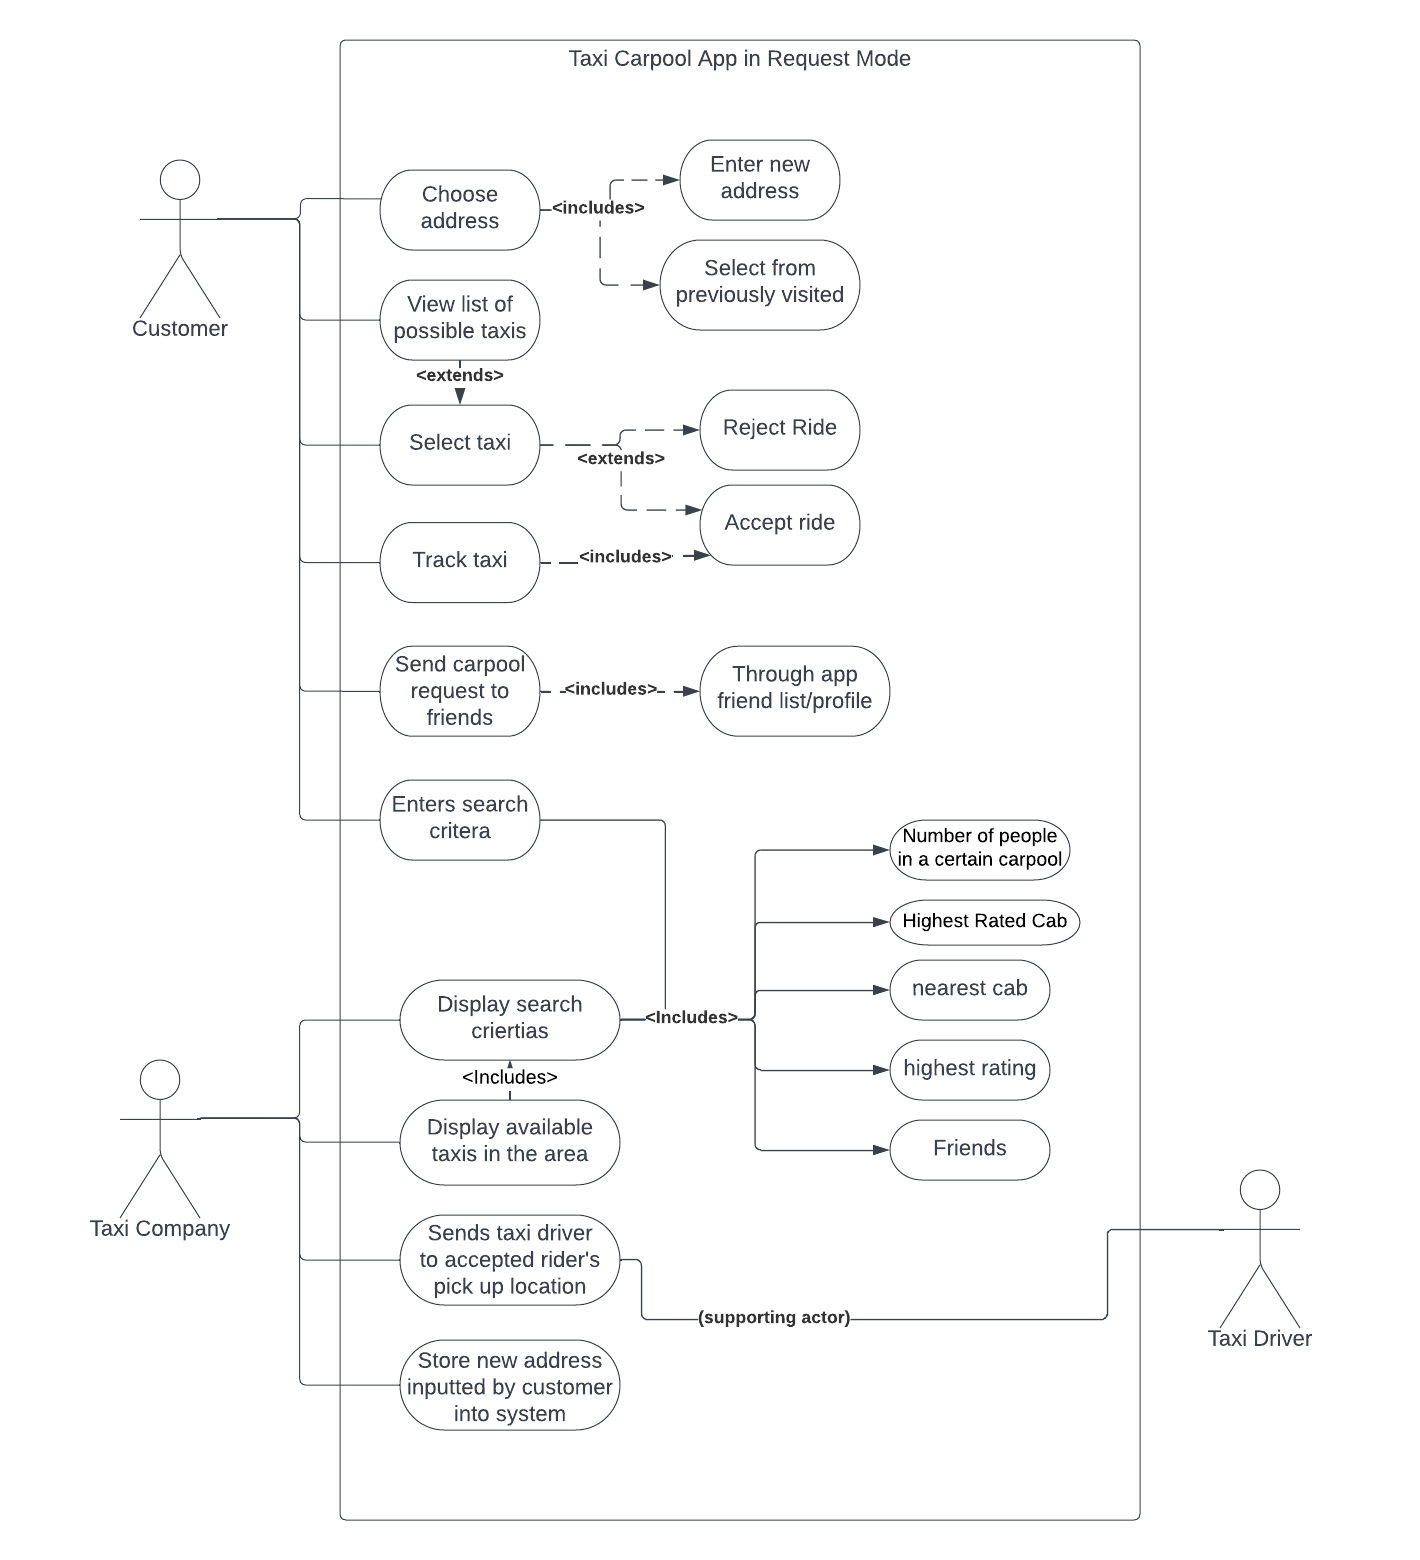
\includegraphics[scale = 0.8]{Use_Case_Diagram.png}

%In this section, select the most important Business Event that your system responds to and give its use case diagram.  Only one use case diagram is needed.  Give a brief textual description of the use case without repeating what is in the scenarios of the corresponding Business Event.

%
%
%
%This section should provide a use case diagram for your application. 
%\begin{enumerate}[a)]
%	\item Each use case appearing in the diagram should be accompanied by a text description. 
%\end{enumerate}
%% End Section

\section{Highlights of Functional Requirements}
\label{sec:functional_requirements}
% Begin Section
\begin{itemize}
	\item Specify the "use cases" organized by Business Event. (The Global Scenario is what you might think of as a use case). Be sure to consider Business Events that aren't just triggered by users with goals (e.g. something happens in the environment that your system needs to respond to)
	\item Your focus should be on what the system needs to do, not how to do it. Specify it in enough detail that it clearly specifies what needs to be accomplished, but not so detailed that you start programming or making design decisions.
	\item Keep the length of each use case (Global Scenario) manageable. If it's getting too long, you need to condense your steps and give a name to what's accomplished by that sequence of steps. (e.g. "Authenticate user" in one line, instead of a list of steps of how to; that's a design decision anyways)
	\item You are \emph{not} specifying a complete and consistent set of functional requirements here. (i.e. you are providing them in the form of use cases/global scenarios, not a refined list). For the purpose of this project, you do not need to reduce them to a list; the global scenarios format is all you need.
\end{itemize}
	Below, we organize by Business Event.
	\begin{enumerate}[{BE}1.]
		\item Business Event name
		\begin{enumerate}[{VP1}.1]
			\item Viewpoint name \newline
			\noindent\fbox{%
				\parbox{0.5\textwidth}{%
					\begin{itemize}
						\item {\bf $S_{1}$:} Initial response of the system to the Business Event
						\item {\bf $E_{1}$:}  Reaction of the environment to $S_{1}$
						\item {\bf $S_{2}$:}  Response of the system to $E_{1}$
						\item {\bf $E_{2}$:}  Reaction of the environment to $S_{2}$
						\item[] $\cdots$
						\item {\bf $S_{n}$:}  Response of the system to $E_{(n-1)}$
						\item {\bf $E_{n}$:}  Reaction of the environment to $E_{(n-1)}$
						\item {\bf $S_{(n+1)}$:} Final response of the system concluding its function regarding the Business Event
					\end{itemize}
				}%
			}
			\item Viewpoint name\newline
			\noindent\fbox{%
				\parbox{0.5\textwidth}{%
					\begin{itemize}
						\item {\bf $S_{1}$:} Initial response of the system to the Business Event
						\item {\bf $E_{1}$:}  Reaction of the environment to $S_{1}$
						\item {\bf $S_{2}$:}  Response of the system to $E_{1}$
						\item {\bf $E_{2}$:}  Reaction of the environment to $S_{2}$
						\item[] $\cdots$
						\item {\bf $S_{k}$:}  Response of the system to $E_{(k-1)}$
						\item {\bf $E_{k}$:}  Reaction of the environment to $E_{(k-1)}$
						\item {\bf $S_{(k+1)}$:} Final response of the system concluding its function regarding the Business Event
					\end{itemize}
				}%
			}
			\item \dots
			\item \dots
			\item \dots
			\item[\dots]
		\end{enumerate}	
		\item[] {\bf Global Scenario of {\it Business Event Name}:} It is the scenario corresponding to the integration of all the above scenarios from the different Viewpoints of the Business Event BE1.\newline
		\noindent\fbox{%
			\parbox{0.5\textwidth}{%
				\begin{itemize}
					\item {\bf $S_{1}$:} Initial response of the system to the Business Event
					\item {\bf $E_{1}$:}  Reaction of the environment to $S_{1}$
					\item {\bf $S_{2}$:}  Response of the system to $E_{1}$
					\item {\bf $E_{2}$:}  Reaction of the environment to $S_{2}$
					\item[] $\cdots$
					\item {\bf $S_{m}$:}  Response of the system to $E_{(m-1)}$
					\item {\bf $E_{m}$:}  Reaction of the environment to $E_{(m-1)}$
					\item {\bf $S_{(m+1)}$:} Final response of the system concluding its function regarding the Business Event
				\end{itemize}
			}%
		}	
		%\end{enumerate}
		\item Business Event name
		\begin{enumerate}[{VP1}.1]
			\item Viewpoint name \newline
			\noindent\fbox{%
				\parbox{0.5\textwidth}{%
					\begin{itemize}
						\item {\bf $S_{1}$:} Initial response of the system to the Business Event
						\item {\bf $E_{1}$:}  Reaction of the environment to $S_{1}$
						\item {\bf $S_{2}$:}  Response of the system to $E_{1}$
						\item {\bf $E_{2}$:}  Reaction of the environment to $S_{2}$
						\item[] $\cdots$
						\item {\bf $S_{n'}$:}  Response of the system to $E_{(n'-1)}$
						\item {\bf $E_{n'}$:}  Reaction of the environment to $E_{(n'-1)}$
						\item {\bf $S_{(n'+1)}$:} Final response of the system concluding its function regarding the Business Event
					\end{itemize}
				}%
			}
			\item Viewpoint name\newline
			\noindent\fbox{%
				\parbox{0.5\textwidth}{%
					\begin{itemize}
						\item {\bf $S_{1}$:} Initial response of the system to the Business Event
						\item {\bf $E_{1}$:}  Reaction of the environment to $S_{1}$
						\item {\bf $S_{2}$:}  Response of the system to $E_{1}$
						\item {\bf $E_{2}$:}  Reaction of the environment to $S_{2}$
						\item[] $\cdots$
						\item {\bf $S_{k'}$:}  Response of the system to $E_{(k'-1)}$
						\item {\bf $E_{k'}$:}  Reaction of the environment to $E_{(k'-1)}$
						\item {\bf $S_{(k'+1)}$:} Final response of the system concluding its function regarding the Business Event
					\end{itemize}
				}%
			}
			\item \dots
			\item \dots
			\item \dots
			\item[\dots]
		\end{enumerate}	
		\item[] {\bf Global Scenario of {\it Business Event Name}:} It is the scenario corresponding to the integration of all the above scenarios from the different Viewpoints of the Business Event BE2.\newline
		\noindent\fbox{%
			\parbox{0.5\textwidth}{%
				\begin{itemize}
					\item {\bf $S_{1}$:} Initial response of the system to the Business Event
					\item {\bf $E_{1}$:}  Reaction of the environment to $S_{1}$
					\item {\bf $S_{2}$:}  Response of the system to $E_{1}$
					\item {\bf $E_{2}$:}  Reaction of the environment to $S_{2}$
					\item[] $\cdots$
					\item {\bf $S_{m'}$:}  Response of the system to $E_{(m'-1)}$
					\item {\bf $E_{m'}$:}  Reaction of the environment to $E_{(m'-1)}$
					\item {\bf $S_{(m'+1)}$:} Final response of the system concluding its function regarding the Business Event
				\end{itemize}
			}%
		}		
	\end{enumerate}

%End Section

\section{Non-Functional Requirements}
\label{sec:non-functional_requirements}


\begin{itemize}
	\item For each non-functional requirement, provide a justification/rationale for it.\\
	{\bf Example:} \\
	SC1. \emph{The device should not explode in a customer’s pocket.}\\
	{\bf Rationale:} Other companies have had issues with the batteries they used in their phones randomly exploding [insert citation]. This causes a safety issue, as the phone is often carried in a person's hand or pocket.	
	\item If you're making a guess because you couldn't really talk to stakeholders, you can say "We imagined stakeholders would want...because..."
	\item Each requirement should have a unique label/number for it.
\end{itemize}

% Begin Section
\subsection{Look and Feel Requirements}
\label{sub:look_and_feel_requirements}
% Begin SubSection

\subsubsection{Appearance Requirements}
\label{ssub:appearance_requirements}
% Begin SubSubSection
\begin{enumerate}[{LF-A}1. ]
	\item 
\end{enumerate}
% End SubSubSection

\subsubsection{Style Requirements}
\label{ssub:style_requirements}
% Begin SubSubSection
\begin{enumerate}[{LF-S}1. ]
	\item 
\end{enumerate}
% End SubSubSection

% End SubSection

\subsection{Usability and Humanity Requirements}
\label{sub:usability_and_humanity_requirements}
% Begin SubSection

\subsubsection{Ease of Use Requirements}
\label{ssub:ease_of_use_requirements}
% Begin SubSubSection
\begin{enumerate}[{UH-EOU}1. ]
	\item 
\end{enumerate}
% End SubSubSection

\subsubsection{Personalization and Internationalization Requirements}
\label{ssub:personalization_and_internationalization_requirements}
% Begin SubSubSection
\begin{enumerate}[{UH-PI}1. ]
	\item 
\end{enumerate}
% End SubSubSection

\subsubsection{Learning Requirements}
\label{ssub:learning_requirements}
% Begin SubSubSection
\begin{enumerate}[{UH-L}1. ]
	\item 
\end{enumerate}
% End SubSubSection

\subsubsection{Understandability and Politeness Requirements}
\label{ssub:understandability_and_politeness_requirements}
% Begin SubSubSection
\begin{enumerate}[{UH-UP}1. ]
	\item 
\end{enumerate}
% End SubSubSection

\subsubsection{Accessibility Requirements}
\label{ssub:accessibility_requirements}
% Begin SubSubSection
\begin{enumerate}[{UH-A}1. ]
	\item 
\end{enumerate}
% End SubSubSection

% End SubSection

\subsection{Performance Requirements}
\label{sub:performance_requirements}
% Begin SubSection

\subsubsection{Speed and Latency Requirements}
\label{ssub:speed_and_latency_requirements}
% Begin SubSubSection
\begin{enumerate}[{PR-SL}1. ]
	\item 
\end{enumerate}
% End SubSubSection

\subsubsection{Safety-Critical Requirements}
\label{ssub:safety_critical_requirements}
% Begin SubSubSection
\begin{enumerate}[{PR-SC}1. ]
	\item 
\end{enumerate}
% End SubSubSection

\subsubsection{Precision or Accuracy Requirements}
\label{ssub:precision_or_accuracy_requirements}
% Begin SubSubSection
\begin{enumerate}[{PR-PA}1. ]
	\item 
\end{enumerate}
% End SubSubSection

\subsubsection{Reliability and Availability Requirements}
\label{ssub:reliability_and_availability_requirements}
% Begin SubSubSection
\begin{enumerate}[{PR-RA}1. ]
	\item 
\end{enumerate}
% End SubSubSection

\subsubsection{Robustness or Fault-Tolerance Requirements}
\label{ssub:robustness_or_fault_tolerance_requirements}
% Begin SubSubSection
\begin{enumerate}[{PR-RFT}1. ]
	\item 
\end{enumerate}
% End SubSubSection

\subsubsection{Capacity Requirements}
\label{ssub:capacity_requirements}
% Begin SubSubSection
\begin{enumerate}[{PR-C}1. ]
	\item 
\end{enumerate}
% End SubSubSection

\subsubsection{Scalability or Extensibility Requirements}
\label{ssub:scalability_or_extensibility_requirements}
% Begin SubSubSection
\begin{enumerate}[{PR-SE}1. ]
	\item 
\end{enumerate}
% End SubSubSection

\subsubsection{Longevity Requirements}
\label{ssub:longevity_requirements}
% Begin SubSubSection
\begin{enumerate}[{PR-L}1. ]
	\item 
\end{enumerate}
% End SubSubSection

% End SubSection

\subsection{Operational and Environmental Requirements}
\label{sub:operational_and_environmental_requirements}
% Begin SubSection

\subsubsection{Expected Physical Environment}
\label{ssub:expected_physical_environment}
% Begin SubSubSection
\begin{enumerate}[{OE-EPE}1. ]
	\item 
\end{enumerate}
% End SubSubSection

\subsubsection{Requirements for Interfacing with Adjacent Systems}
\label{ssub:requirements_for_interfacing_with_adjacent_systems}
% Begin SubSubSection
\begin{enumerate}[{OE-IA}1. ]
	\item 
\end{enumerate}
% End SubSubSection

\subsubsection{Productization Requirements}
\label{ssub:productization_requirements}
% Begin SubSubSection
\begin{enumerate}[{OE-P}1. ]
	\item 
\end{enumerate}
% End SubSubSection

\subsubsection{Release Requirements}
\label{ssub:release_requirements}
% Begin SubSubSection
\begin{enumerate}[{OE-R}1. ]
	\item 
\end{enumerate}
% End SubSubSection

% End SubSection

\subsection{Maintainability and Support Requirements}
\label{sub:maintainability_and_support_requirements}
% Begin SubSection

\subsubsection{Maintenance Requirements}
\label{ssub:maintenance_requirements}
% Begin SubSubSection
\begin{enumerate}[{MS-M}1. ]
	\item 
\end{enumerate}
% End SubSubSection

\subsubsection{Supportability Requirements}
\label{ssub:supportability_requirements}
% Begin SubSubSection
\begin{enumerate}[{MS-S}1. ]
	\item 
\end{enumerate}
% End SubSubSection

\subsubsection{Adaptability Requirements}
\label{ssub:adaptability_requirements}
% Begin SubSubSection
\begin{enumerate}[{MS-A}1. ]
	\item 
\end{enumerate}
% End SubSubSection

% End SubSection

\subsection{Security Requirements}
\label{sub:security_requirements}
% Begin SubSection

\subsubsection{Access Requirements}
\label{ssub:access_requirements}
% Begin SubSubSection
\begin{enumerate}[{SR-AC}1. ]
	\item 
\end{enumerate}
% End SubSubSection

\subsubsection{Integrity Requirements}
\label{ssub:integrity_requirements}
% Begin SubSubSection
\begin{enumerate}[{SR-INT}1. ]
	\item 
\end{enumerate}
% End SubSubSection

\subsubsection{Privacy Requirements}
\label{ssub:privacy_requirements}
% Begin SubSubSection
\begin{enumerate}[{SR-P}1. ]
	\item 
\end{enumerate}
% End SubSubSection

\subsubsection{Audit Requirements}
\label{ssub:audit_requirements}
% Begin SubSubSection
\begin{enumerate}[{SR-AU}1. ]
	\item 
\end{enumerate}
% End SubSubSection

\subsubsection{Immunity Requirements}
\label{ssub:immunity_requirements}
% Begin SubSubSection
\begin{enumerate}[{SR-IM}1. ]
	\item 
\end{enumerate}
% End SubSubSection

% End SubSection

\subsection{Cultural and Political Requirements}
\label{sub:cultural_and_political_requirements}
% Begin SubSection

\subsubsection{Cultural Requirements}
\label{ssub:cultural_requirements}
% Begin SubSubSection
\begin{enumerate}[{CP-C}1. ]
	\item 
\end{enumerate}
% End SubSubSection

\subsubsection{Political Requirements}
\label{ssub:political_requirements}
% Begin SubSubSection
\begin{enumerate}[{CP-P}1. ]
	\item 
\end{enumerate}
% End SubSubSection

% End SubSection

\subsection{Legal Requirements}
\label{sub:legal_requirements}
% Begin SubSection

\subsubsection{Compliance Requirements}
\label{ssub:compliance_requirements}
% Begin SubSubSection
\begin{enumerate}[{LR-COMP}1. ]
	\item 
\end{enumerate}
% End SubSubSection

\subsubsection{Standards Requirements}
\label{ssub:standards_requirements}
% Begin SubSubSection
\begin{enumerate}[{LR-STD}1. ]
	\item 
\end{enumerate}
% End SubSubSection

% End SubSection

% End Section

\appendix
\section{Division of Labour}
\label{sec:division_of_labour}
% Begin Section
Include a Division of Labour sheet which indicates the contributions of each team member. This sheet must be signed by all team members.
% End Section

\newpage
\section*{IMPORTANT NOTES}
\begin{itemize}
	\item Be sure to include all sections of the template in your document regardless whether you have something to write for each or not
	\begin{itemize}
		\item If you do not have anything to write in a section, indicate this by the \emph{N/A}, \emph{void}, \emph{none}, etc.
	\end{itemize}
	\item Uniquely number each of your requirements for easy identification and cross-referencing
	\item Highlight terms that are defined in Section~1.3 (\textbf{Definitions, Acronyms, and Abbreviations}) with \textbf{bold}, \emph{italic} or \underline{underline}
	\item For Deliverable 1, please highlight, in some fashion, all (you may have more than one) creative and innovative features. Your creative and innovative features will generally be described in Section~2.2 (\textbf{Product Functions}), but it will depend on the type of creative or innovative features you are including.
\end{itemize}


\end{document}
%------------------------------------------------------------------------------